% Insert: image of latin text "M. AVR. AVG. LIB."
% Traced the source:
% Out of Rome - Inscription outside the wall of the Church at Civita Lavinia,
% dedicated by the Senate and people of Lanvinium to M. AVRELIVS AGILIVS.
% SEPTENTRIONI, (AD 180). 
% http://quod.lib.umich.edu/k/kelsey/x-2000.01.2380/1
% http://www.theatrum.de/508.html says:
% "Ehreninschrift des Pantomimen M. Aurelius Agilius Septentrio,
%  CIL XIV 2113 (187 n.Chr.)"
% [translation: Inscription to honor the panromime M. Aurelius Agillius
%  Septentrio, CIL XIV 2113 (187 CE)]
% M(arco) Aur(elio) Aug(usti) lib(erto)
% Agilio Septentrioni
% pantomimo sui
% temporis primo(.) sacerdoti
% synhodi apollinis parasito
% alumno Faustinae
% Aug(ustae) producto ab Imp(eratore) M(arco)
% Aurel(io) <<Commodo>> Antonino
% Pio Felice Augusto
% ornamentis decurionat(us)
% decreto ordinis exornato
% et allecto inter iuvenes
% S(enatus) P(opulus)Q(ue) Lanivinus
% [A latere dextro saxi] [tr: on the right side of the stone:]
% [---] Idus Commodas
% [---]eliano co(n)s(ulibus)
%%
% "Marco Aurelio Augusti"
% tr: Dedicated to Marcus Aurelio Augustus
% "liberto Agilio Septentrioni"
% tr: liberated slave of Agilius of the North.
% "pantomimo sui temporis primo."
% tr: The best pantomime (dancer who performs all roles) of his time.
% "Sacerdoti synhodi apollonis parasito."
% tr: Guest at the table of the synod of the priests of Apollo
% "Alumno Faustinae Augustae."
% tr: Fostered by Faustina the Younger (daughter of Emperor Antoninus Pius,
%     wife of Emperor Marcus Aurelius, mother of Emperor Commodus).
% "Producto ab Imperatore Marco Aurelio Commodo, Antonino Pio Felice, Augusto,
% ornamentis(decorations, dative/ablative) decurionatus(local official)
% decreto(decree) ordinis(of the group, class, order, station, rank)
% exornato(he adorned)"
% tr: Produced by decree of Emperor Marcus Aurelius Commodo,
%     [?] the blessing of Antoninus Pio (his grandfather), Augustus,
%     by the group of the decurionatus (local  official)...
%     Maybe: given the title and decorations of decurionatus?
%     
% et allecto inter iuvenes
% tr: [?] and popular among the young?
% "S.P.Q. Lanivinus"
% tr: By the senate and the people or Lanivinus
% "A latere dextro saxi"
% tr: on the right side of the stone:
%% ==> This is why this illustration is in this book
% "Idus Commodas Eliano consulibus"
% tr: The ides of the month of Commodus Aelius, consul, i.e. the 13th of August
%% ===
\begin{figure}[t]
  \centering
  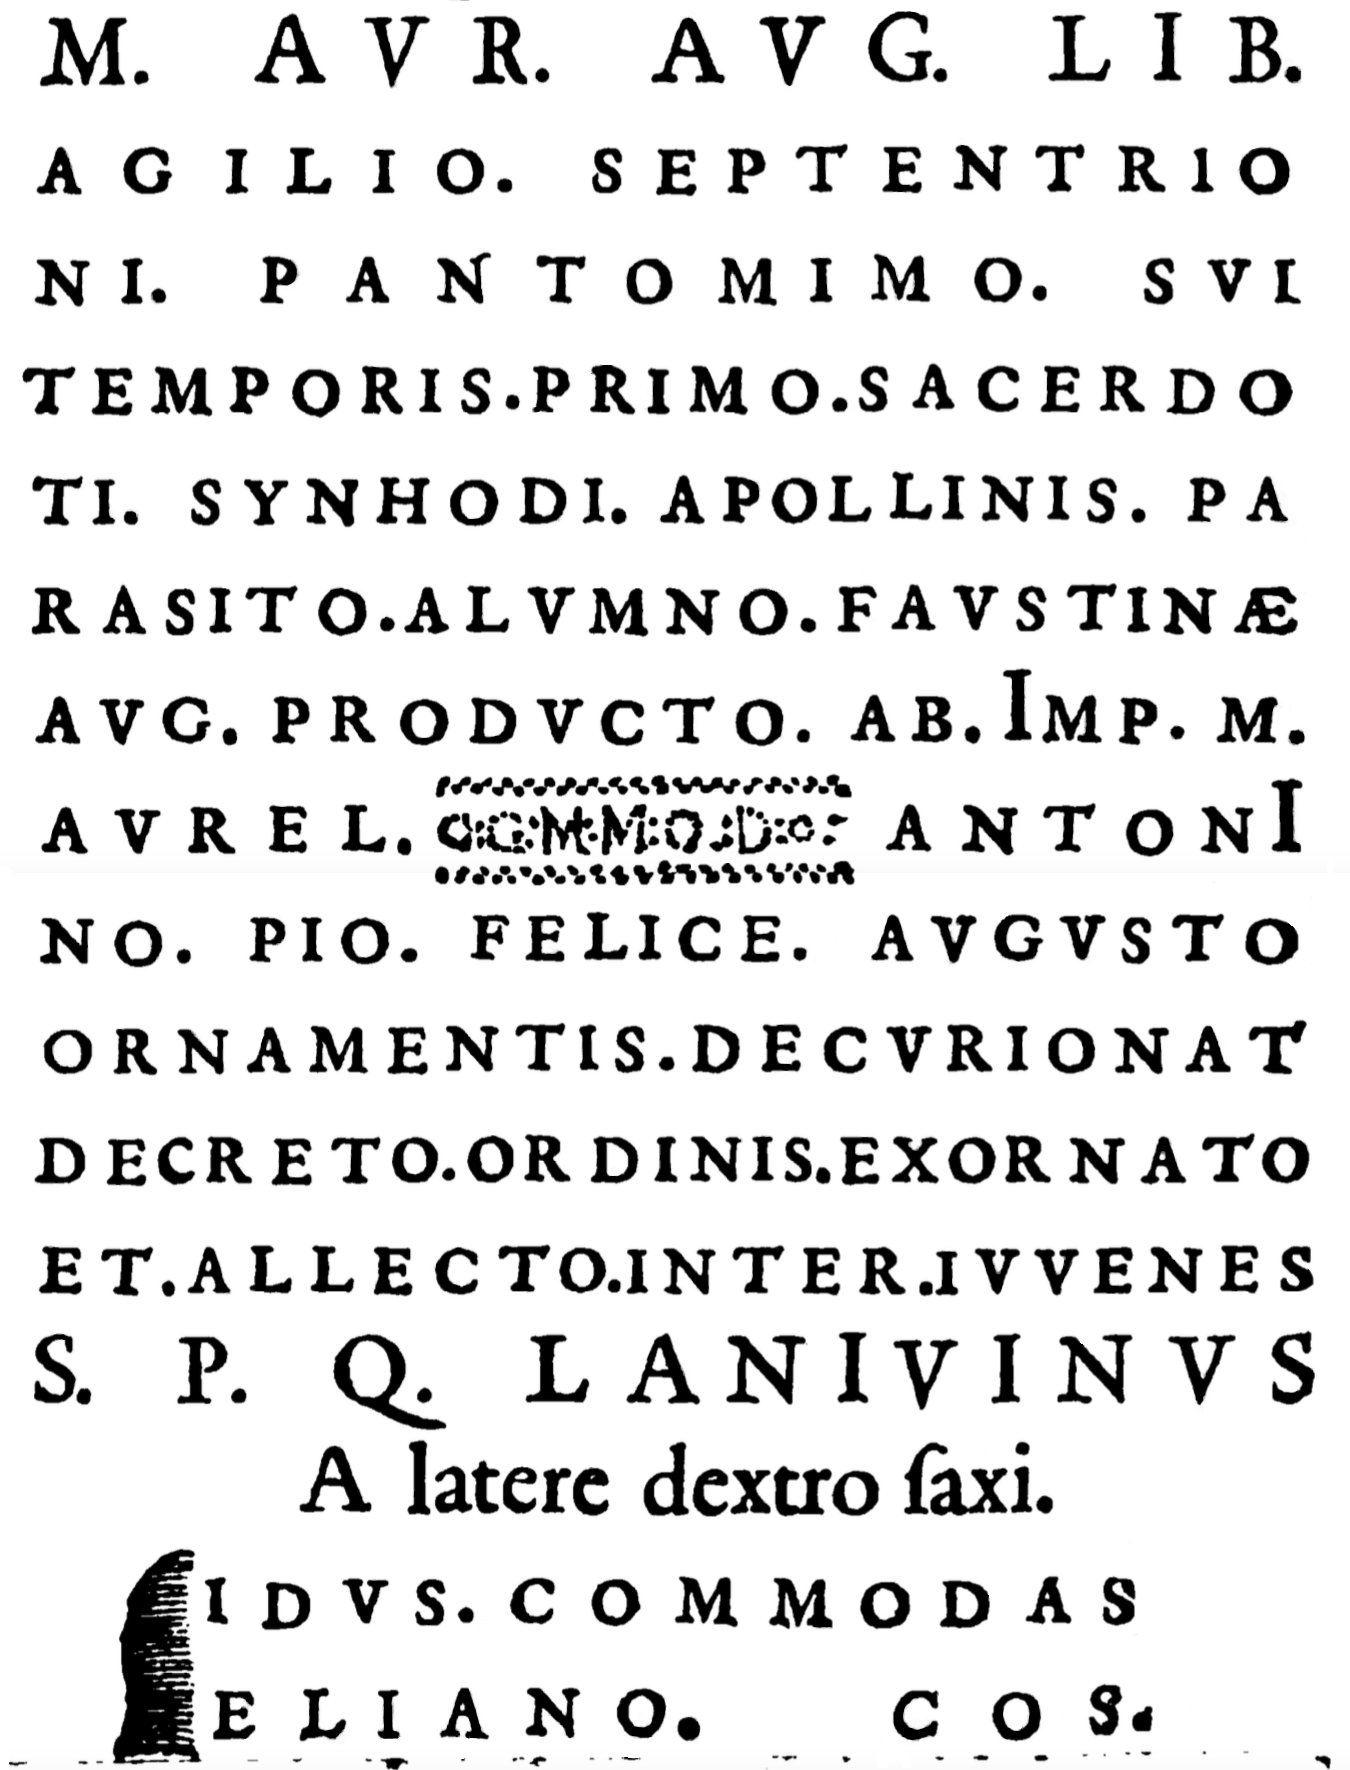
\includegraphics[width=0.5\textwidth]{lapis_lavinii}
  \caption{Lapis Lavinii}
  \label{fig:lapis_lavinii}
\end{figure}
